\subsection{Template Method}
\label{template-method}

\textbf{Scopo}: Comportamentale \\
\textbf{Raggio d'azione}: Classi

\paragraph{Definizione} Il pattern definisce la struttura di un algoritmo all'interno di un metodo, delegando alcuni passi alle sottoclassi (motivo per cui è un pattern class-based).

Consente, introducendo sottoclassi diverse, di cambaire il modo in cui i sottopassi vengono eseguiti, lasciando inalterata la struttura dell'algoritmo che è stato inglobato.

\paragraph{Motivazione} Considera un framework applicativo che fornisce classi Application e Document, dove la classe Application è responsabile di aprire documenti esistenti memorizzati in un formato esterno come un file, e un oggetto Document rappresenta le informazioni in un documento una volta che è stato letto dal file. Le applicazioni costruite con il framework possono creare sottoclassi di Application e Document per soddisfare bisogni specifici: per esempio, un'applicazione di disegno definisce sottoclassi DrawApplication e DrawDocument, mentre un'applicazione foglio di calcolo definisce sottoclassi SpreadsheetApplication e SpreadsheetDocument. La classe astratta Application definisce l'algoritmo per aprire e leggere un documento nella sua operazione OpenDocument che definisce ogni passo per aprire un documento: controlla se il documento può essere aperto, crea l'oggetto Document specifico dell'applicazione, lo aggiunge al suo insieme di documenti, e legge il Document da un file. Chiamiamo OpenDocument un template method, che definisce un algoritmo in termini di operazioni astratte che le sottoclassi sovrascrivono per fornire comportamento concreto, dove le sottoclassi Application definiscono i passi dell'algoritmo che controllano se il documento può essere aperto (CanOpenDocument) e che creano il Document (DoCreateDocument), mentre le classi Document definiscono il passo che legge il documento (DoRead).

\begin{figure}[H]
    \centering
    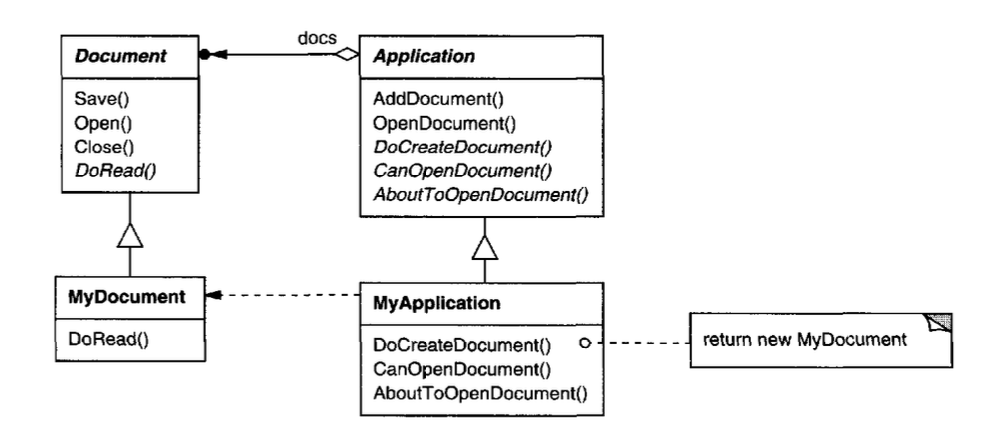
\includegraphics[width=0.75\linewidth]{assets/pattern/template-method/template-esempio.png}
\end{figure}

Il template method definisce anche un'operazione che permette alle sottoclassi Application di sapere quando il documento sta per essere aperto (AboutToOpenDocument), nel caso sia di loro interesse. Definendo alcuni dei passi di un algoritmo usando operazioni astratte, il template method fissa il loro ordine, ma permette alle sottoclassi Application e Document di variare quei passi per soddisfare i loro bisogni.

\paragraph{Applicabilità} Il pattern Template Method è utile quando:
\begin{itemize}
    \item Si desidera implementare una volta sola le parti invarianti di un algoritmo e lasciare alle sottoclassi l'implementazione dei comportamenti che possono variare.
    \item I comportamenti comuni tra le sottoclassi devono essere fattorizzati e localizzati in una classe comune per evitare la duplicazione del codice;
    \item Si vogliono controllare le estensioni delle sottoclassi;
\end{itemize}

\begin{figure}[H]
    \centering
    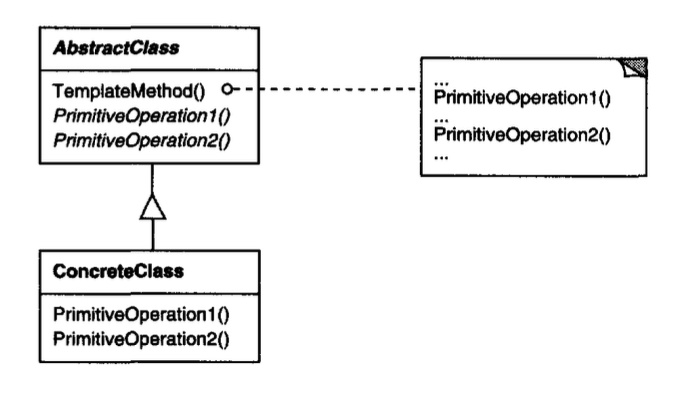
\includegraphics[width=0.5\linewidth]{assets/pattern/template-method/template-struttura.png}
    \caption{Class Diagram del pattern Template}
\end{figure}

\paragraph{Struttura} Il pattern è composto da:
\begin{itemize}
    \item \textbf{AbstractClass} (Applicazione): definisce operazioni primitive astratte che le sottoclassi concrete definiscono per implementare le fasi di un algoritmo.Implementa un metodo modello che definisce lo scheletro di un algoritmo. Il metodo modello richiama operazioni primitive, operazioni definite in AbstractClass o quelle di altri oggetti.
    \item \textbf{ConcreteClass} (MyApplication): implementa le operazioni primitive per eseguire le fasi dell'algoritmo specifiche della sottoclasse.
\end{itemize}

ConcreteClass si basa su AbstractClass per implementare i passaggi invarianti dell'algoritmo.

\begin{figure}[H]
    \centering
    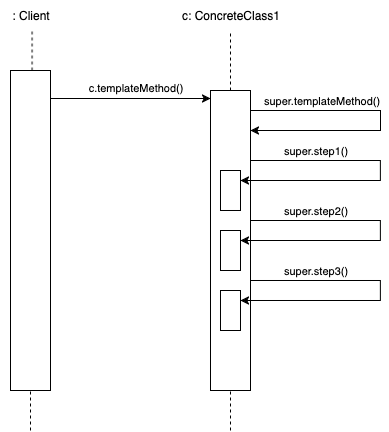
\includegraphics[width=0.5\linewidth]{assets/pattern/template-method/template-sequence.drawio.png}
    \caption{Sequence Diagram del pattern Template}
\end{figure}

\paragraph{Conseguenze} Il pattern Template Method consente quindi di:
\begin{itemize}
    \item Riutilizzare codice già scritto;
    \item Applicare il \textbf{principio di Hollywood} (Don't call us, we'll call you): la classe padre chiama le operazioni di una sottoclasse e non viceversa;
\end{itemize}

Il pattern permette di rimuovere codice duplicato inserendolo nella AbstractClass, però alcuni client potrebbero essere limitati dallo scheletro fornito di un dato algoritmo. In più i metodi tendono ad essere più difficili da mantenere all'aumentare dei passaggi forniti.



\newpage